\documentclass[letterpaper,12pt]{article}

\usepackage{subfigure}
\usepackage{setspace}
\usepackage{color}
\usepackage{graphicx}
\usepackage{fullpage}
\usepackage{times}
\usepackage{amsmath}
\usepackage{amssymb}
\usepackage{textcomp}
\usepackage{mathpazo}
\usepackage{verbatim}
\usepackage{listings}
\usepackage{xcolor}
\usepackage{natbib}
\usepackage{algorithm2e}
\usepackage{enumitem}
\usepackage{amsmath,tikz}
\usetikzlibrary{matrix}
\def\SPSB#1#2{\rlap{\textsuperscript{\textcolor{red}{#1}}}\SB{#2}}
\def\SP#1{\textsuperscript{\textcolor{red}{#1}}}
\def\SB#1{\textsubscript{\textcolor{blue}{#1}}}
\setlist{noitemsep} % or \setlist{noitemsep} to leave space around whole list

\linespread{1}


% abbreviations
\usepackage{xspace}
\makeatletter
\DeclareRobustCommand\onedot{\futurelet\@let@token\@onedot}
\def\@onedot{\ifx\@let@token.\else.\null\fi\xspace}
\def\eg{{e.g}\onedot} \def\Eg{{E.g}\onedot}
\def\ie{{i.e}\onedot} \def\Ie{{I.e}\onedot}
\def\cf{{c.f}\onedot} \def\Cf{{C.f}\onedot}
\def\etc{{etc}\onedot}
\def\vs{{vs}\onedot}
\def\wrt{w.r.t\onedot}
\def\dof{d.o.f\onedot}
\def\etal{{et al}\onedot}
\makeatother
\definecolor{orange}{rgb}{1,0.55,0}

\lstset{	language=c++,
			basicstyle=\footnotesize\ttfamily, 
			stepnumber=1,
			tabsize=2,
			frame=shadowbox, 
			rulesepcolor=\color{blue}}
			
\title{2D Schr\"{o}dinger Dynamics Simulation}
\author{Sean Hatch, PHY 480}
\begin{document}


	\renewcommand{\topfraction}{0.9}	% max fraction of floats at top
    \renewcommand{\bottomfraction}{0.8}	% max fraction of floats at bottom
    %   Parameters for TEXT pages (not float pages):
    \setcounter{topnumber}{2}
    \setcounter{bottomnumber}{2}
    \setcounter{totalnumber}{2}     % 2 may work better
    \setcounter{dbltopnumber}{2}    % for 2-column pages
    \renewcommand{\dbltopfraction}{0.9}	% fit big float above 2-col. text
    \renewcommand{\textfraction}{0.07}	% allow minimal text w. figs
    %   Parameters for FLOAT pages (not text pages):
    \renewcommand{\floatpagefraction}{0.7}	% require fuller float pages
	% N.B.: floatpagefraction MUST be less than topfraction !!
    \renewcommand{\dblfloatpagefraction}{0.7}	% require fuller float pages


\maketitle

\section{Introduction and Goals}

For this project, our basic goal is to numerically simulate a Gaussian wave packet in a two-dimensional domain using the time-dependent Schr\"{o}dinger's equation:
\begin{equation}
\begin{split}
- \frac{1}{2}\nabla^2 \psi(\mathbf{r},t) + V(r)\psi(\mathbf{r},t) = \mathrm{i}\hbar\partial_t\psi(\mathbf{r},t)
\end{split}
\end{equation}

Where the wave packet is initialized to:

\begin{equation}
\begin{split}
\psi(\mathbf{r},t = 0) = \mu\exp( - \frac{(\mathbf{r} - \mathbf{r_0})^2}{2\sigma^2} )*\exp(\mathrm{i}\mathbf{k}\cdot\mathbf{r})
\end{split}
\end{equation}


We use reference \citep{reference} as a starting point. In \citep{reference}, the authors described the requisite numerical methods used to perform the simulation, and matched some canonical results.

For this work, we will develop only a two-dimensional model, and try to validate our code against the reference work.  In particular, we chose to replicate the following experiments: (1) Free propagation of Gaussian wave packet, (2) Gaussian wave packet normally incident upon a potential barrier, and (3) Young's double-slit experiment. 

\section{Algorithm Details}

\citep{reference} introduces the numerical methods used to solve the problem at hand, and some details about them are described here.

\subsection{Time-Stepping Schemes}

To perform the time-stepping for the simulation, three schemes were suggested: (1) A forward Euler method, (2) a Runge-Kutta method, and (3) the Crank-Nicholson scheme. Two of the three were implemented for the present project, and some details will be discussed below.

\subsubsection{Euler Method}

This method uses a center difference for the spatial second-order derivatives, and a forward difference for the time step.  For the one-dimensional Schr\"{o}dinger's equation, this scheme results in the following update equation:

\begin{equation}
\begin{split}
\frac{-\delta t}{2i\delta x^2}\psi^n_{i-1} + 
\frac{-\delta t}{2i\delta x^2}\psi^n_{i+1} +
( \frac{\delta t}{i\delta x^2} + \frac{\delta t} {i}V^n_{i} + 1)\psi^n_{i}  = \psi^{n+1}_{i} 
\end{split}
\end{equation}

Since this is an explicit finite-difference scheme, the time step must be chosen carefully to ensure stability in the simulation. The maximum time step to ensure stability can be rigorously derived (see, for example \citep{eulerstab}), but for now, we will just use time steps of about 1e-6, as suggested by \citep{reference}.

The two-dimensional Euler scheme is listed below:

\begin{equation}
\begin{split}
\frac{-\delta t}{2i\delta x^2}\psi^n_{i-1,j} + 
\frac{-\delta t}{2i\delta x^2}\psi^n_{i+1,j} +
\frac{-\delta t}{2i\delta y^2}\psi^n_{i,j-1} + 
 \frac{-\delta t}{2i\delta y^2}\psi^n_{i,j+1} + \\ 
(  \frac{\delta t}{i\delta x^2} + \frac{\delta t}{i\delta y^2} + \frac{\delta t} {i}V^n_{i,j} + 1)\psi^n_{i,j}  = \psi^{n+1}_{i,j} 
\end{split}
\end{equation}

For the present work, the stability requirement proved too prohibitive to produce any meaningful or high resolution results. The method was implemented in the code, but was not used to generate any of the results.

\subsubsection{Runge-Kutta method}

The authors of \citep{reference} presented a Runge-Kutta method as a time-stepping scheme.  In theory, the accuracy of this scheme allows for larger timesteps, and many of the results in \citep{reference} were generated with this scheme.

However, I was a bit skeptical of some aspects of this scheme:

\begin{itemize}
  \item The stages of the RK4 method presented in \citep{reference} all appear to use samples from $\psi^{n-1}$ -- the wave function at the previous time step. The canonical method uses three different points in time to compute the stages. 
  \item In general, computing the stages of the RK4 method appear to require spatial interpolation, since the right hand side is itself computed from a finite difference scheme. This also may lead to diminished accuracy.
\end{itemize}

Furthermore, the implementation of this method can be more challenging to implement if $\psi$ is stored with a data type similar to C++'s std::complex, as opposed to a code where real and imaginary arrays are stored separately.

(Okay, I probably just don't understand this method too well, or was confused by the notation).


\subsubsection{Crank-Nicholson method}

The Crank-Nicholson method is an implicit method, where, essentially, the time derivative (ie, $\psi^{n+1}$) is computed based on an average of spatial derivatives from the current time step, and the next time step. This scheme, in theory, has no stability requirement, but we are at the mercy of obtaining an accurate matrix solution. A good introduction to this method can be found in \citep{heat}.  After some algebra, we come to the update equation listed below:
  
\begin{equation}
\begin{split}
\frac{-\delta t}{4i\delta x^2}\psi^n_{i-1,j} + 
\frac{-\delta t}{4i\delta x^2}\psi^n_{i+1,j} +
\frac{-\delta t}{4i\delta y^2}\psi^n_{i,j-1} + 
 \frac{-\delta t}{4i\delta y^2}\psi^n_{i,j+1} + \\ 
(  \frac{\delta t}{2i\delta x^2} + \frac{\delta t}{2i\delta y^2} + \frac{\delta t} {2i}V^n_{i,j} + 1)\psi^n_{i,j} + \\
 \frac{-\delta t}{4i\delta x^2}\psi^{n+1}_{i-1,j} + 
 \frac{-\delta t}{4i\delta x^2}\psi^{n+1}_{i+1,j} + 
\frac{-\delta t}{4i\delta y^2}\psi^{n+1}_{i,j-1} + 
 \frac{-\delta t}{4i\delta y^2}\psi^{n+1}_{i,j+1} + \\ 
(  \frac{\delta t}{2i\delta x^2} + \frac{\delta t}{2i\delta y^2} + \frac{\delta t} {2i}V^{n+1}_{i,j} -1)\psi^{n+1}_{i,j} = 0 
\end{split}
\end{equation}

Clearly, we cannot update each $\psi$ independently, so a matrix solution is required to compute the update. The required matrix equation is shown below.

\begin{equation}
\begin{tikzpicture}[baseline=(current bounding box.center)]
\matrix (m) [matrix of math nodes,nodes in empty cells,right delimiter={]},left delimiter={[} ]{
1 &  & && & &  & &  \\
& 1 &  & && & &  & &  \\
\ddots & \ddots & \ddots & \ddots & \ddots & \ddots &\ddots & \ddots & \ddots \\
c & \cdots & b	&	a_{1,1}	& b &	\cdots & c  & \cdots & \cdots \\
\cdots & c & \cdots & b	&	a_{2,1}	& b &	\cdots & c  & \cdots \\
\ddots & \ddots & \ddots & \ddots & \ddots & \ddots &\ddots & \ddots & \ddots \\
} ;\end{tikzpicture}
\begin{pmatrix}
\psi^{n+1}_{0,0} \\ \psi^{n+1}_{1,0}\\\vdots\\ \psi^{n+1}_{0,1} \\ \psi^{n+1}_{1,1} \\\vdots  
\end{pmatrix}=
\begin{pmatrix}
d^{n}_{0,0} \\ d^{n}_{1,0}\\\vdots\\ d^{n}_{0,1} \\ d^{n}_{1,1} \\\vdots  
\end{pmatrix}
\label{eq:eqq1}
\end{equation}

The RHS of this equation consists of the terms of equation (5) from the previous timestep.  

The coefficient matrix can be difficult to visualize, and some subtleties are worth discussing.  First, the ones along the diagonal enforce the boundary condition that the next value of $\psi$ is equal to the previous value of $\psi$ on the boundaries.  These rows are not needed in the matrix, but including them ensures that the coefficients $a_{i,j}$ remain on the diagonal of the matrix.  This is important, since these values are often larger in magnitude than $b$ and $c$, so this matrix is more likely to be diagonally-dominant, or at least close to it.  For diagonally-dominant matrices, a simple matrix-splitting technique, like a Jacobi iteration, can solve the matrix equation. However, for the present work, conjugate gradient turned out to be the solution method of choice.

Note that the vector $\psi^{n+1}$ reflects the "x-major" storage used to store the domain.   

The coefficients used in the above matrix equation are shown below.
\begin{equation}
\begin{split}
c = \frac{-\delta t}{4i\delta x^2} \\
b = \frac{-\delta t}{4i\delta y^2} \\
a_{i,j} = (  \frac{\delta t}{2i\delta x^2} + \frac{\delta t}{2i\delta y^2} + \frac{\delta t} {2i}V^{n+1}_{i,j} - 1) \\
d_{i,j} = 	\frac{-\delta t}{4i\delta x^2}\psi^n_{i-1,j} + 
			\frac{-\delta t}{4i\delta x^2}\psi^n_{i+1,j} +
			\frac{-\delta t}{4i\delta y^2}\psi^n_{i,j-1} + 
 			\frac{-\delta t}{4i\delta y^2}\psi^n_{i,j+1} + \\ 
			(  \frac{\delta t}{2i\delta x^2} + \frac{\delta t}{2i\delta y^2} + \frac{\delta t} 				{2i}V^n_{i,j} + 1)\psi^n_{i,j}\\
\end{split}
\end{equation}

Finally, here are a few other notes about obtaining the matrix solution:
\begin{itemize}
  \item From these equations, we see that $a_{i,j}$ has terms of differing sign, so we cannot be sure that the coefficient matrix is diagonally-dominant.
  \item In general, for iterative matrix solvers, we must start with an initial guess.  The matrix solution may converge more quickly if the supplied guess is the solution from the last time-step (which will be somewhat similar to the solution for the next time-step). However, the solution becomes less similar to that of the previous time step as our time step increases.  In the end, a balance should be struck between these two factors.
  \end{itemize}

\subsection{Boundary Conditions}

For any finite difference simulation, boundary conditions must be considered.  The authors of \citep{reference} chose to setup an exponential potential wall around the periphery of the domain to create a potential well.  The present work uses the same method, and the potential is initialized based on the following equation:

\begin{equation}
\begin{split}
V_{i,j} = c( \exp(a(idy-y_L) + \exp(a(jdx-x_L) + \exp(-aidy) + \exp(-a j dx) )
\end{split}
\end{equation}

Where the parameters $a$ and $c$ are chosen somewhat experimentally.  A term like $idy$ is simply the y coordinate of the $i$'th row of the domain.   
   
\section{\bf Commented Source Code}

All of the source code used for the project is posted below.  Each listing
is commented, and further explanation will be given afterwards.

\begin{lstlisting}[caption=Domain header].
#ifndef DOM
#define DOM

#include <complex>
#include <iostream>
#include <iomanip>
#include <fstream>
#include "matrix.h"

using namespace std;


struct node_data
{
	double V;
	complex<double> psi;
};


class domain
{
	typedef std::complex<double> comp_t;
	typedef dat<complex<double> > dat_t;

public:

	domain(int rows, int cols, double dx, double dy);

	~domain()
	{
		//delete cn_A;
		//delete cn_b;
		//delete cn_x;
	}

	//utility
	void		allocate_nodes();
	void		dump(ostream &str);
	void		dump_separate(string prefix);
	inline int	idx(int i, int j){	return i*cols_+j; }
	void		copy_to_last();
	
	//potential
	void make_barrier(double V0, double x0, double x1, double y0, double y1);
	void make_wall_barrier(double a, double c);

	void gauss_barrier_y(	double y0, double x0, double x1, 
								double a, double b, double c);
	void gauss_barrier_x(	double x0, double y0, double y1, 
								double a, double b, double c);
	
	//integrators
	void timestep_euler(double dt);
	void timestep_cranknicholson(double dt);
	void cn_init(double dt);
	
	//other
	double	psi_sum();
	void	init_psi(double kx, double ky, double sigma, double x0, double y0);
	
	
	//members
	double		dx_;
	double		dy_;
	int			rows_; //diff. by dy
	int			cols_; //diff. by dx
	node_data**	d_; 
	node_data** d_last_;

	cmat< complex<double> >*		cn_b;
	cmat< complex<double> >*		cn_x;
	cmat< complex<double> >*		cn_A;
		

};
#endif

\end{lstlisting}
\vspace{5 mm}

The domain class abstracts the information related to the simulation domain.  It contains most of the key data, the finite difference schemes, and methods to set up the initial potentials in the domain.  Also note that the key simulation data ($\psi$ and $V$) are stored node-wise in a struct.

\vspace{5 mm}

\begin{lstlisting}[caption=Domain class implementation].
#include "domain.h"

domain::domain(int rows, int cols, double dx, double dy):
	  rows_(rows),cols_(cols),dx_(dx),dy_(dy)
	{	
		//domain constructor
		cn_A = NULL;	//new cmat(rows*cols,rows*cols);
		cn_b = NULL;	//new cmat(rows*cols,1);
		cn_x = NULL;	//new cmat(rows*cols,1);  
	  
	 }

void domain::allocate_nodes()
{
	//allocate domain, and another data
	//vector to store the previous timestep
	d_ =		new node_data*[rows_*cols_];
	d_last_ =	new node_data*[rows_*cols_];
		
	for(int i = 0; i < rows_*cols_; i++)
	{
		d_[i] =			new node_data;
		d_[i]->psi =	comp_t(0.,0.);
		d_[i]->V =		0.;		

		d_last_[i] =		new node_data;
		d_last_[i]->psi =	comp_t(0.,0.);
		d_last_[i]->V =		0.;
	}

	printf("* Domain allocated.  Mem. required is about: %i kB\n",
		((rows_*cols_)*(sizeof(void*) + sizeof(node_data)))/1000 );

	printf("* Total cells is: %i \n",
		rows_*cols_);

}

void domain::dump(ostream &str)
{
	//Print domain items to the specified
	//stream, str.

	cout << "Printing Psi: \n";
	for(int i = 0; i < rows_; i++){
		for(int j = 0; j < cols_; j++){
			str << setw(25) << d_[i*cols_+j]->psi;
		}
		str << "\n";
	}

	str << "Printing V: \n";
	for(int i = 0; i < rows_; i++){
		for(int j = 0; j < cols_; j++){
			str << setw(15) << d_[i*cols_+j]->V;
		}
		str << "\n";
	}
}

void domain::dump_separate(string prefix)
{
	//Print some files related to the domain

	string v_name = prefix + "_potential.txt";
	string psi_name_r = prefix + "_psi_real.txt";
	string psi_name_im = prefix + "_psi_imag.txt";
	string psi_mag_name = prefix + "_psi_mag.txt";

	ofstream f;
	f.open(v_name.c_str() );
		
	for(int i = 0; i < rows_; i++){
		for(int j = 0; j < cols_; j++){
			f << setw(20) << d_[i*cols_+j]->V;
		}
		f << "\n";
	}
		
	f.close();

	f.open(psi_name_r.c_str());
	for(int i = 0; i < rows_; i++){
		for(int j = 0; j < cols_; j++){
			f << setw(20) << d_[i*cols_+j]->psi.real();
		}
		f << "\n";
	}

	f.close();
		
	f.open(psi_name_im.c_str());
	for(int i = 0; i < rows_; i++){
		for(int j = 0; j < cols_; j++){
			f << setw(20) << d_[i*cols_+j]->psi.imag();
		}
		f << "\n";
	}

	f.close();


	f.open(psi_mag_name.c_str());
	for(int i = 0; i < rows_; i++){
		for(int j = 0; j < cols_; j++){
			f << setw(20) << abs(d_[i*cols_+j]->psi)*abs(d_[i*cols_+j]->psi);
		}
		f << "\n";
	}
	f.close();

}

void domain::make_wall_barrier(double a, double c)
{
	
	//This function creates potential well which acts as the boundary
	//condition
	for(int i = 0; i < rows_; i++){
		for(int j = 0; j < cols_; j++){
		
			d_[i*cols_+j]->V += c * (	exp( a*(i*dy_ - dy_*(rows_-1))) +//				;// +											
										exp( a*(j*dx_ - dx_*(cols_-1))) +//; //+// +
										exp( -1.*a*(j*dx_))  +//  +//;
										exp( -1.*a*(i*dy_)) ); 
		}
	}
}

void domain::copy_to_last()
{
	//set d_last_ = d_
	for(int i = 0; i < rows_*cols_; i++)
	{
		d_last_[i]->V =		d_[i]->V;
		d_last_[i]->psi =	d_[i]->psi;
	}
}
void domain::timestep_euler(double dt)
{
	//do euler timestep with stepsize dt

	//alias swap
	std::swap(d_last_,d_);
	
	comp_t a = -1.*(dt/ (2.*comp_t(0,1.)*dx_*dx_) );
	comp_t b = -1.*(dt/ (2.*comp_t(0,1.)*dy_*dy_) );		
	comp_t c = dt/(2.*comp_t(0,1.));
		
	int ilast, inext, jlast, jnext;

	for(int i = 0; i < rows_; i++)
	{
		ilast = i-1; inext = i+1;
		for(int j = 0; j < cols_; j++)
		{			
			jlast = j-1; jnext = j+1;
				
			//do nothing at the boundaries, or set them to zero
			//(this is nearly equivalent)
			if(i == 0 || j ==0 || i == rows_-1 || j == cols_-1)
			{}//	d_[idx(i,j)]->psi = 0.;
			else
			{		

				d_[idx(i,j)]->psi = b*d_last_[idx(ilast,j)]->psi + 
									b*d_last_[idx(inext,j)]->psi +
									a*d_last_[idx(i,jlast)]->psi + 
									a*d_last_[idx(i,jnext)]->psi +
									2.*(-a + -b + c*d_last_[idx(i,j)]->V + 0.5)*d_last_[idx(i,j)]->psi;	
			}
		}
	}	
}

void domain::timestep_cranknicholson(double dt)
{
	//Do Crank Nicholson timestep
	//alias swap
	std::swap(d_last_,d_);
	
	comp_t a = -1.*(dt/ (4.*comp_t(0,1.)*dx_*dx_) );
	comp_t b = -1.*(dt/ (4.*comp_t(0,1.)*dy_*dy_) );		
	comp_t c = dt/(2.*comp_t(0,1.));	
	
	//malloc x and b
	comp_t* x_vect = new comp_t[rows_*cols_];
	comp_t* b_vect = new comp_t[rows_*cols_];
	
	//create b
	for(int i = 0; i < rows_; i++)
	{
		for(int j = 0; j < cols_; j++)
		{

			if(i == 0 || j ==0 || i == rows_-1 || j == cols_-1)
				b_vect[i*cols_ + j] = d_last_[idx(i,j)]->psi;
			else
				b_vect[i*cols_ + j] = -1.*(	b*d_last_[idx(i-1,j)]->psi + 
											b*d_last_[idx(i+1,j)]->psi +
									  		a*d_last_[idx(i,j-1)]->psi + 
									  		a*d_last_[idx(i,j+1)]->psi +
											(-2.*a + -2.*b + c*d_last_[idx(i,j)]->V + 1.)*
												d_last_[idx(i,j)]->psi	);

		}
	}
	
	//make guess from d_last
	for(int i = 0; i < rows_*cols_; i++)
		x_vect[i] = d_last_[i]->psi;

	//cg solve
	cn_A->cg(x_vect,b_vect,200);
	
	//copy solution to d_
	for(int i = 0; i < rows_*cols_; i++)
		d_[i]->psi = x_vect[i];
		
	//cleanup (we should just make these class members)
	delete[] x_vect;
	delete[] b_vect;
		
}

void domain::cn_init(double dt)
{
	//initialize banded Crank Nicholson matrix

	comp_t a = -1.*(dt/ (4.*comp_t(0,1.)*dx_*dx_) );
	comp_t b = -1.*(dt/ (4.*comp_t(0,1.)*dy_*dy_) );		
	comp_t c = dt/(2.*comp_t(0,1.));
	
	comp_t self_term;

	cn_A = new cmat<comp_t>();
	
	for(int i = 0; i < rows_; i++)
	{
		for(int j = 0; j < cols_; j++)
		{
			//add a new sparse row
			cn_A->new_row();
			
			//enforce d_next = d on edges
			if(i == 0 || j ==0 || i == rows_-1 || j == cols_-1)
				cn_A->mat_data_.push_back( dat_t(comp_t(1.,0),i*cols_ + j) );
			//fill in matrix bands
			else
			{
				self_term = (-2.*a + -2.*b + c*d_[i*cols_+j]->V - 1.);

				cn_A->mat_data_.push_back( dat_t(self_term,i*cols_+j) );
				
				cn_A->mat_data_.push_back( dat_t(a,i*cols_+j +1) );
				cn_A->mat_data_.push_back( dat_t(a,i*cols_+j -1) );
				
				cn_A->mat_data_.push_back( dat_t(b,i*cols_+j + cols_) );
				cn_A->mat_data_.push_back( dat_t(b,i*cols_+j - cols_) );

			}			
		}
	}
	
	printf("* CN Matrix allocated, mem. required is about: %i kB\n",
			(cn_A->mat_data_.size()*(16 + 4))/1000);
}

double domain::psi_sum()
{
	//Compute Norm
	double sum = 0;

	for(int i = 0; i < rows_; i++)
	{
		for(int j = 0; j < cols_; j++)
		{
			sum += abs(d_[idx(i,j)]->psi)*abs(d_[idx(i,j)]->psi)*dx_*dy_;
		}
	}
	return sum;
}

void domain::init_psi(double kx, double ky, double sigma, double x0, double y0)
{

	double x,y,dist2,kr;
	for(int i = 0; i < rows_; i++){
			
		y = i*dy_;				
		for(int j = 0; j < cols_; j++){
				
			x =		j*dx_;
			dist2 = (x-x0)*(x-x0) + (y-y0)*(y-y0);
			kr =	kx*x + ky*y;				
			d_[i*cols_+j]->psi = 5*exp( -1.*dist2 /(2*sigma*sigma) )*exp(comp_t(0.,kr));
			
		}
	}

}

void domain::gauss_barrier_y(	double y0, double x0, double x1, 
								double a, double b, double c)
{
	//cols_ .. x
	//rows_ .. y

	int x_start = int( x0 / dx_ );
	int x_end = ceil((x1 / dx_));

	for(int i = x_start; i < x_end; i++)
	{
		for(int j = 0; j < cols_; j++)
		{
			d_[idx(i,j)]->V += a*exp( -( (j*dy_-b)*(j*dy_-b) / (2.*c*c) ) );
		}
	}
}

void domain::gauss_barrier_x(	double x0, double y0, double y1, 
								double a, double b, double c)
{
	//cols_ .. x
	//rows_ .. y

	int y_start = int( y0 / dy_ );
	int y_end = ceil((y1 / dy_));

	for(int i = y_start; i < y_end; i++) //dy
	{
		for(int j = 0; j < cols_; j++)
		{
			d_[idx(i,j)]->V += a*exp( -( (j*dx_-b)*(j*dx_-b) / (2.*c*c) ) );
		}
	}
}
\end{lstlisting}

\vspace{5 mm}

The most important part of the domain class is the implementation of the numerical schemes from section 2. The method $domain::time\_stepeuler()$ implements the Euler method.  The method $domain::cn\_init()$ sets up the sparse coefficient matrix (see eq.(6)), and $timestep\_cranknicholson()$ sets up and solves the matrix equation at each time step.

Also, note that functions such as $domain::gauss\_barrier\_x()$ can be used to specify a potential barrier at a given x-coordinate with specified y-extents.  Therefore, this function can be used as a sort of building block to create more complex potentials.  For example, we can setup the potential used for the double-slit experiment with three calls to this function.
\vspace{5 mm}

\begin{lstlisting}[caption=sparse matrix class template].
#ifndef cmatX
#define cmatX

#include <vector>
#include <complex>
#include <iostream>
#include <cstring>

using namespace std;

/////////////////////////
//Sparse Data Member
////////////////////////

template<class T>
class dat
{
public:

	dat(T x, int col):
	  x_(x),col_(col){}

	T	x_;
	int	col_;	
};

/////////////////////////
//Sparse Matrix Class
////////////////////////


template<class T>
class cmat
{
	public:
		
		//Sparse matrix data vector and 
		//row index vector
		vector< dat<T>  > 	mat_data_;
		vector< int > 		row_idx_;			
	
		//auxilliary vectors
		T*	diag_table_;
		T*	x_extra;

		cmat();
		~cmat(){/*delete diag_table_*/}
		void print();
		void insert( dat<T> k, int i, int j);
				
		//vector operations
		static complex<double> 	vect_dot( complex<double>* a, 
			complex<double>* b, int n);
		static void vect_add( T* a, T* b, T* res, T alpha, int n);
		static void vect_sub( T* a, T* b, T* res, T alpha, int n);
		static void vect_copy( T* a, T* b, int n);
		
		//Math functions: conjugate gradient, jacobi,
		//and matrix vector product
		void cg(T* x, T* b, int iters);
		void jacobi(T* x, T* b, int iters);
		void mv( T* x, T* b);
		
		void new_row();	//add a new row to the sparse matrix
		inline int m(); //get size of (square) sparse matrix
		
		//make vector of diagonal elements of matrix
		void make_diag_table();
		void get_range(int &start, int &end, int i);
		
		//debug, etc.
		void print_full(ostream &outStr);
		double print_norm(T* a, T* b, int n, int k);
		static void print_dense_vector(T* x, int n, string desc = "");
		
	
};

template<class T>
cmat<T>::cmat():
	x_extra(NULL)
{}
	
template<class T>	
void cmat<T>::print()
{

	int start_idx,end_idx;
	for(unsigned int i = 0 ; i < row_idx_.size() ; i ++ )
	{							
		get_range(start_idx,end_idx,i);

		cout << "row: " << i << endl;
		for(int j = start_idx ; j < end_idx+1; j++)
			cout << "(" << mat_data_[j].col_ <<"-->" << mat_data_[j].x_ << ")" << endl;
					
		cout << endl;
	}
}

template<class T>		
void cmat<T>::insert( dat<T> k, int i, int j)
{
			///////////////
			//insert data k at A(i,j)
			//////////////
}

template<class T>
void cmat<T>::print_dense_vector(T* x, int n, string desc)
{
	cout << "Printing vector: " << desc << endl;
	for(int i =0; i < n; i++)
		cout << x[i] << endl;

	cout << endl;
}

template<class T>
void cmat<T>::make_diag_table()
{
	//it is up to the user to make sure
	//a diag exists
	//for each row	
	diag_table_ = new T[row_idx_.size()];
	int start_idx,end_idx;

	for(int i = 0 ; i < int(row_idx_.size()) ; i ++ )
	{							
		get_range(start_idx,end_idx,i);

		//it would actually be more efficient to 
		//do the diag term and then subtract it later
		for(int j = start_idx ; j < end_idx+1; j++)
		{
			if(mat_data_[j].col_ == i)
				diag_table_[i] = mat_data_[j].x_; 
		}
	}
}


template<class T>
void cmat<T>::get_range(int &start, int &end, int i)
{
	start	= row_idx_[i];
		
	if(i != int(row_idx_.size()) - 1)	end =  row_idx_[i+1] - 1;
	else								end = mat_data_.size() - 1;
}

template<class T>		
complex<double> cmat<T>::vect_dot( complex<double>* a, 
	complex<double>* b, int n)
{			
	complex<double> sum = 0;
	for(int i =0; i < n ;i++)
		sum += a[i]*conj(b[i]);
		
	return sum;		
}

template<class T>
void cmat<T>::vect_add( T* a, T* b, T* res, T alpha, int n)
{
	//a + b
	for(int i = 0; i < n ;i++)
		res[i] = a[i] + alpha*b[i];
}

template<class T>
void cmat<T>::vect_sub( T* a, T* b, T* res, T alpha, int n)
{
	//a - b
	for(int i = 0; i < n ;i++)
		res[i] = a[i] - alpha*b[i];
}		

template<class T>
void cmat<T>::vect_copy( T* a, T* b, int n)
{
	//dest,src,size in bytes
	memcpy(a,b,sizeof(T)*n);			
}

template<class T>
void cmat<T>::cg(T* x, T* b, int iters)
{
	
	double tol = 1e-6;
	
	T* r_cur = 		new T[m()];
	T* r_next = 	new T[m()];
	T* p = 			new T[m()];
	T* temp_Ap = 	new T[m()];
	T alpha,beta,rr_cur,rr_next;
	//last values for x and p not needed
	
	//init

	vect_copy(r_cur,b,m());
	mv(x,temp_Ap);
	vect_sub(r_cur,temp_Ap,r_cur,1.,m());
	vect_copy(p,r_cur,m());
	
	rr_cur = vect_dot(r_cur,r_cur,m());
	
	
	for(int i = 0; i < iters; i++)
	{							
		
		mv(p,temp_Ap); //Ap=A*p
		alpha = rr_cur / vect_dot(p,temp_Ap,m());
	
		vect_add(x,p,x,alpha,m());
		vect_sub(r_cur,temp_Ap,r_next,alpha,m());
		
		rr_next = vect_dot(r_next,r_next,m());
		
		beta = rr_next / rr_cur;
		
		if(iters % 100 == 0)
			//cout << "Res: " << rr_next << endl;
		if( sqrt(abs(rr_next)) < tol) 
			break;
	
		vect_add(r_next,p,p,beta,m());
	
		//next mv and update
		swap(r_cur,r_next);
		rr_cur = rr_next;
	} 
	
	delete[] r_cur;
	delete[] r_next;
	delete[] p;
	delete[] temp_Ap;
			
}

template<class T>
void cmat<T>::print_full(ostream &outstr)
{
	cout << setprecision(4);
	int start_idx,end_idx;
	int rows = m();
	
	for(int i = 0 ; i < rows; i ++ )
	{							
	
		get_range(start_idx,end_idx,i);

		for(int j = 0; j < rows; j++)
		{
			bool found  = false;
			for(int k = start_idx ; k < end_idx+1; k++)
			{
			
				if(mat_data_[k].col_ == j)
				{
					outstr << setw(15) << mat_data_[k].x_;
					found = true;
					break;
				}
			}
			
			if(!found)	
				outstr << setw(15) << T(0);			
		}
		
		outstr << endl;
	}
}

template<class T>
void cmat<T>::jacobi(T* x, T* b, int iters)
{
	int start_idx,end_idx;
	int rows = m();
	double convergence;
	
	if(!x_extra) 
		x_extra = new T[row_idx_.size()];

	for(int k = 0 ; k < iters ; k++ )
	{				
		for(int i = 0 ; i < rows; i ++ )
		{							
			T sigma = b[i];
			get_range(start_idx,end_idx,i);

			//it would actually be more efficient to 
			//do the diag term and then subtract it later
			for(int j = start_idx ; j < end_idx+1; j++)
			{
				if(mat_data_[j].col_ != i)
					sigma -= mat_data_[j].x_*x[mat_data_[j].col_];
			}
	
			x_extra[i] = sigma / diag_table_[i];
		
		}

		swap(x,x_extra);			
		if( k > 10 && k % 10 == 0)
		{
			if(print_norm(x,x_extra,row_idx_.size(),k) < 1e-12)
			{	
				cout << "Solution converged." << endl;
				break;
			}
		}
		//print_dense_vector(x,row_idx_.size() );
	
	}	
}

template<class T>
void cmat<T>::new_row()
{
	row_idx_.push_back( mat_data_.size() );
}

template<class T>
void cmat<T>::mv( T* x, T* b)
{
	//b is dest
	int start_idx,end_idx;
	
	for(int i=0;i<int(row_idx_.size());i++)
	{
		get_range(start_idx,end_idx,i);
		
		b[i] = 0;	
		for(int j = start_idx; j < end_idx+1; j++)
			b[i] += mat_data_[j].x_ * x[ mat_data_[j].col_ ];       									
	}			
}

template<class T>
double cmat<T>::print_norm(T* a, T* b, int n, int k)
{
	double sum =0;
	for(int i = 0; i < n; i++)
		sum += abs(a[i] - b[i])*abs(a[i] - b[i]);

	sum = sqrt(sum);
	cout << "Convergence at iteration " << k << " " << sum << endl;
	return sum;
}

template<class T>
inline int cmat<T>::m(){ return row_idx_.size(); }

#endif
\end{lstlisting}

\vspace{5 mm}

The code above is a class template for sparse matrix operations.  Templating this class is probably excessive for the current project, but this template can now be used in any other project requiring sparse matrix operations, without much modification.

Most of the methods in the class essentially help us implement the sparse conjugate gradient method, or the sparse Jacobi iteration, one of which is required to solve the matrix equation required for the Crank-Nicholson update. 

Much of the functionality found in this class is already implemented elsewhere in third-party libraries, but I wrote my own to keep debugging and building simple.
  
\vspace{5 mm}

\begin{lstlisting}[caption=examples.h].
#ifndef UTIL_1
#define	UTIL_1

#include "examples.h"
#include "matrix.h"
#include "domain.h"


namespace examples
{


	void matrix_test()
	{
		typedef cmat<complex<double> > cmatcd;
		typedef dat<complex<double> > datcd;
		/////////////
		//test for cmat class
		/////////////
		cmat<complex<double> > A;

		A.row_idx_.push_back(0);
		A.mat_data_.push_back( datcd(3.2,0) );
		A.mat_data_.push_back( datcd(0.2,2) );
		A.mat_data_.push_back( datcd(0.2,4) );


		A.new_row();
		A.mat_data_.push_back( datcd(0.5,0) );
		A.mat_data_.push_back( datcd(2.2,1) );
		A.mat_data_.push_back( datcd(0.2,3) );

		A.new_row();
		A.mat_data_.push_back( datcd(0.8,1) );
		A.mat_data_.push_back( datcd(1.2,2) );

		A.new_row();
		A.mat_data_.push_back( datcd(0.2,1) );
		A.mat_data_.push_back( datcd(5.2,3) );

		A.new_row();
		A.mat_data_.push_back( datcd(0.6,3) );
		A.mat_data_.push_back( datcd(8.2,4) );
		

		A.print();
		A.print_full(cout);
		complex<double>* b = new complex<double>[A.m()];
		complex<double>* x = new complex<double>[A.m()];

		//x is guess
		for(int i =0; i < A.m(); i++)
		{
			x[i] = complex<double>(1,0);
			b[i] = complex<double>(1,0);
		}

		A.make_diag_table();
		A.cg(x,b,20);

		A.print_dense_vector(x,A.m());
		
		A.mv(x,b);
		A.print_dense_vector(b,A.m());
	}


	void matrix_test2()
	{
		typedef cmat<complex<double> > cmatcd;
		typedef dat<complex<double> > datcd;
		typedef std::complex<double> comp_t;
		typedef dat<complex<double> > dat_t;
		
		int n = 2000;
		/////////////
		//test for cmat class
		/////////////
		cmat<complex<double> > A;
		
		complex<double> a = 2.65;
		complex<double> bb = 0.5;
		complex<double> c = 0.1;
	
		//
		for(int i = 0; i < n ; i++)
		{
			for(int j = 0; j < n ; j++)
			{
				//add a new sparse row
				A.new_row();			
			
				if(i == 0 || j ==0 || i == n-1 || j == n-1)
					A.mat_data_.push_back( dat_t(comp_t(1.,0),i*n + j) );
				//fill in matrix bands
				else
				{			
					A.mat_data_.push_back( dat_t(a,i*n+j) );
					
					A.mat_data_.push_back( dat_t(bb,i*n+j +1) );
					A.mat_data_.push_back( dat_t(bb,i*n+j -1) );
					
					A.mat_data_.push_back( dat_t(c,i*n+j + n) );
					A.mat_data_.push_back( dat_t(c,i*n+j - n) );
				}
			}			
		}
		
		//A.print();
		//A.print_full();
		
		complex<double>* b = new complex<double>[A.m()];
		complex<double>* x = new complex<double>[A.m()];

		//x is guess
		for(int i =0; i < A.m(); i++)
		{
			x[i] = complex<double>(1,0);
			b[i] = complex<double>(1,0);
		}

		A.make_diag_table();
		//A.jacobi(x,b,50);
		A.cg(x,b,50);
		//A.print_dense_vector(x,A.m());
		
		A.mv(x,b);
		//A.print_dense_vector(b,A.m());
	}
	void setup_potential(){}

	void run_cn2()
	{
	
		/////////////////////////
		//Free Prop. Experiment
		////////////////////////

		double dx =		.025;
		double dy =		.005;
		double x_max =	1;
		double y_max =	1.5;
		double dt =		12.5e-6;
		double n =		20000;
		vector<double> norms;
		double normloss;
	
		domain* mydom = new domain(int(y_max/dy),int(x_max/dx),dx,dy);
		mydom->allocate_nodes();
		mydom->init_psi(0,20,.1,x_max/2,y_max/3);
		
		//exp(1x) * 10
		mydom->make_wall_barrier(5.,30);		
		mydom->copy_to_last();
		mydom->cn_init(dt);

		for(int i = 0; i < n; i++)
		{			
			mydom->timestep_cranknicholson(dt);
			if(i % 100 == 0)
			{
				cout << "\n++++++++++++\nStep: " << i << endl;
				norms.push_back( mydom->psi_sum());
				normloss = ( (norms[norms.size()-1] - norms[0]) / norms[0])*100;
				cout << "Norm Loss is: " << normloss << "%" << endl;

				mydom->dump_separate( string( "output_step" + 
					to_string( (long long) i) +"_") );
			}
		}
	}

	void run_cn3()
	{
	
		/////////////////////////
		//Potential Barrier/Tunneling Experiment
		////////////////////////

		double dx =		.01;
		double dy =		.01;
		double x_max =	1.5;
		double y_max =	1;
		double dt =		5e-6;
		double n =		20000;
		vector<double> norms;
		double normloss;
		
		domain* mydom = new domain(int(y_max/dy),int(x_max/dx),dx,dy);
		mydom->allocate_nodes();
		mydom->init_psi(20,0,.1,x_max/3,y_max/2);
		
		//exp(1x) * 10
		mydom->make_wall_barrier(5.,30);
		
		//Make potential barrier and init.
		//Crank-Nicholson Matrix, A
		mydom->gauss_barrier_x(x_max/2,0,y_max,1e3,x_max/2,.01);
		mydom->copy_to_last();
		mydom->cn_init(dt);

		//do timestepping
		for(int i = 0; i < n; i++)
		{			
			mydom->timestep_cranknicholson(dt);
		
			if(i % 100 == 0)
			{
				cout << "\n++++++++++++\nStep: " << i << endl;
				norms.push_back( mydom->psi_sum());
				normloss = ( (norms[norms.size()-1] - norms[0]) / norms[0])*100;
				cout << "Norm Loss is: " << normloss << "%" << endl;

				mydom->dump_separate( string( "output_step" + 
					to_string( (long long) i) +"_") );
			}
		}
	}

	void run_cn4()
	{

		/////////////////////////
		//Double Slit Experiment
		////////////////////////
			
		double dx =		.01;
		double dy =		.01;
		double x_max =	2.5;
		double y_max =	4;
		double dt =		10e-6;
		double n =		20000;
		double k =		60;
		double aperature_size = (2*3.14159) / k;
		vector<double> norms;
		double normloss;
		
		domain* mydom = new domain(int(y_max/dy),int(x_max/dx),dx,dy);
		mydom->allocate_nodes();
		mydom->init_psi(k,0,.2,x_max/3,y_max/2);
		
		//exp(1x) * 10
		mydom->make_wall_barrier(5.,30);
		
		//Make the double slit:
		mydom->gauss_barrier_x(x_max/2,0,y_max/2-1.5*aperature_size,1e3,x_max/2,.015);
		mydom->gauss_barrier_x(x_max/2,y_max/2+1.5*aperature_size,y_max,1e3,x_max/2,.015);
		mydom->gauss_barrier_x(x_max/2,y_max/2-0.5*aperature_size,y_max/2+0.5*aperature_size,1e3,x_max/2,.015);
				
		mydom->copy_to_last();
		mydom->cn_init(dt);

		for(int i = 0; i < n; i++)
		{			
			mydom->timestep_cranknicholson(dt);
			
			if(i % 100 == 0)
			{
				cout << "\n++++++++++++\nStep: " << i << endl;
				norms.push_back( mydom->psi_sum());
				normloss = ( (norms[norms.size()-1] - norms[0]) / norms[0])*100;
				cout << "Norm Loss is: " << normloss << "%" << endl;

				mydom->dump_separate( string( "output_step" + to_string( (long long) i) +"_") );
			}
		}
	}
}

#endif
\end{lstlisting}

\vspace{5mm}

The examples namespace just contains functions that perform some of the numerical experiments from \citep{reference}.  We will use these examples to validate the code. These functions and the simulations that they perform are further discussed in the next section.

\vspace{5mm}

\section{Results and Discussion} 

For now, we will simply try to re-create some results from \citep{reference}.

\subsection{Free Propagation of Gaussian Wave-packet}

First, we try to re-create free propagation.  The propagation is not strictly 'free', since we have initialized a potential 'bowl' near the edge of the domain as our boundary condition.  This experiment can be run with the function $examples::run\_cn2()$ from the supplied source-code. Listed below are some parameters for the simulation:

\begin{center}
    \begin{tabular}{ | l | l  |}
    \hline
    Parameter & Value  \\ \hline
	$k_x$ & 0  \\ \hline
	$k_y$ & 20  \\ \hline    
	$\delta t$ & 12.5e-6  \\ \hline    
    $\delta x$ & .025  \\ \hline    
    $\delta y$ & .005  \\ \hline    
    Solver & Conjugate Gradient  \\ \hline            
    \hline
    \end{tabular}
\end{center}

The results from the simulation can be seen in Figures \ref{fig:p1} - \ref{fig:p3}.  These results show very good agreement with the reference work.

\begin{figure}[!htbp]
\centering
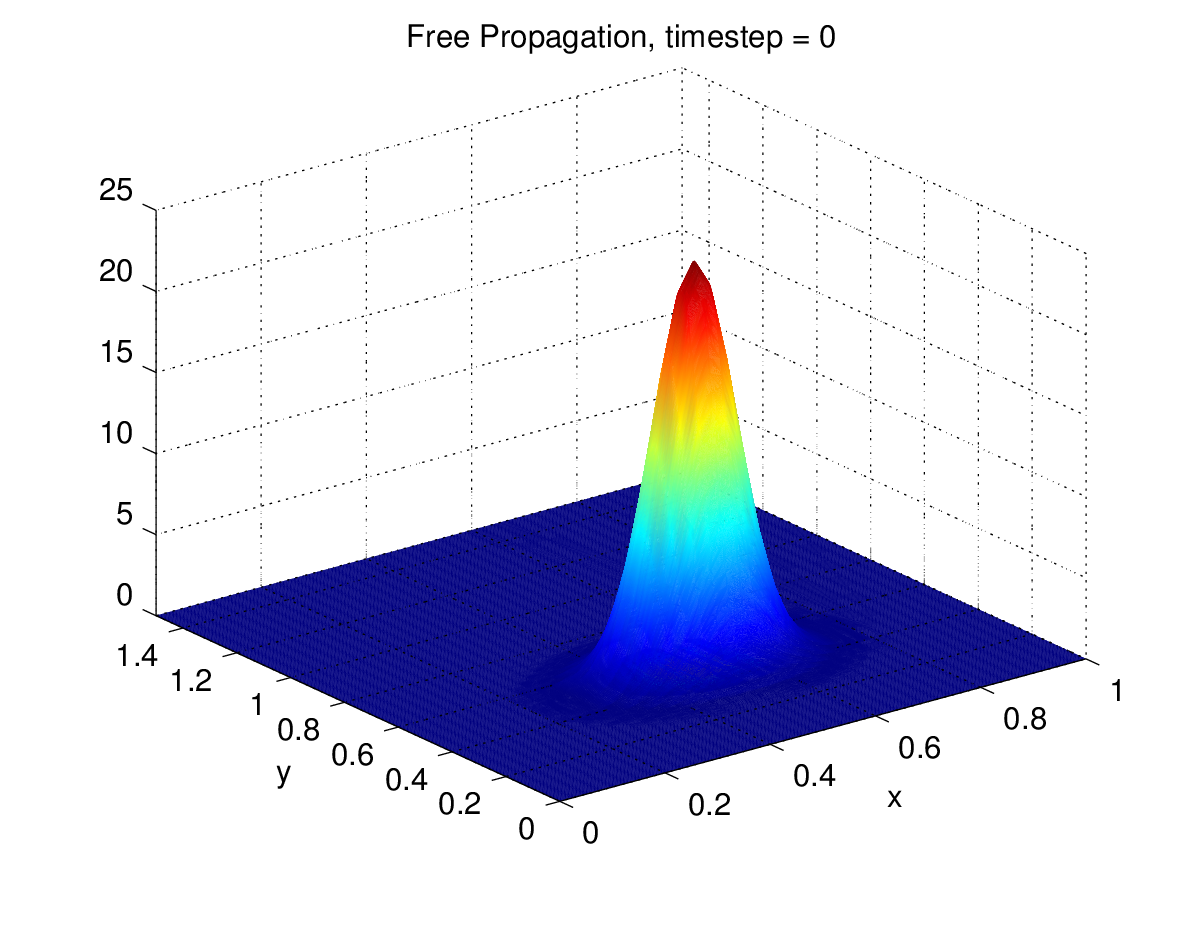
\includegraphics[scale=0.55,trim = 2mm 12mm 12mm 2mm,clip=true]{prop1.png}
\caption{Free propagation, time step = 0 (See Figure 9 from \citep{reference}).}
\label{fig:p1}
\end{figure}

\begin{figure}[!htbp]
\centering
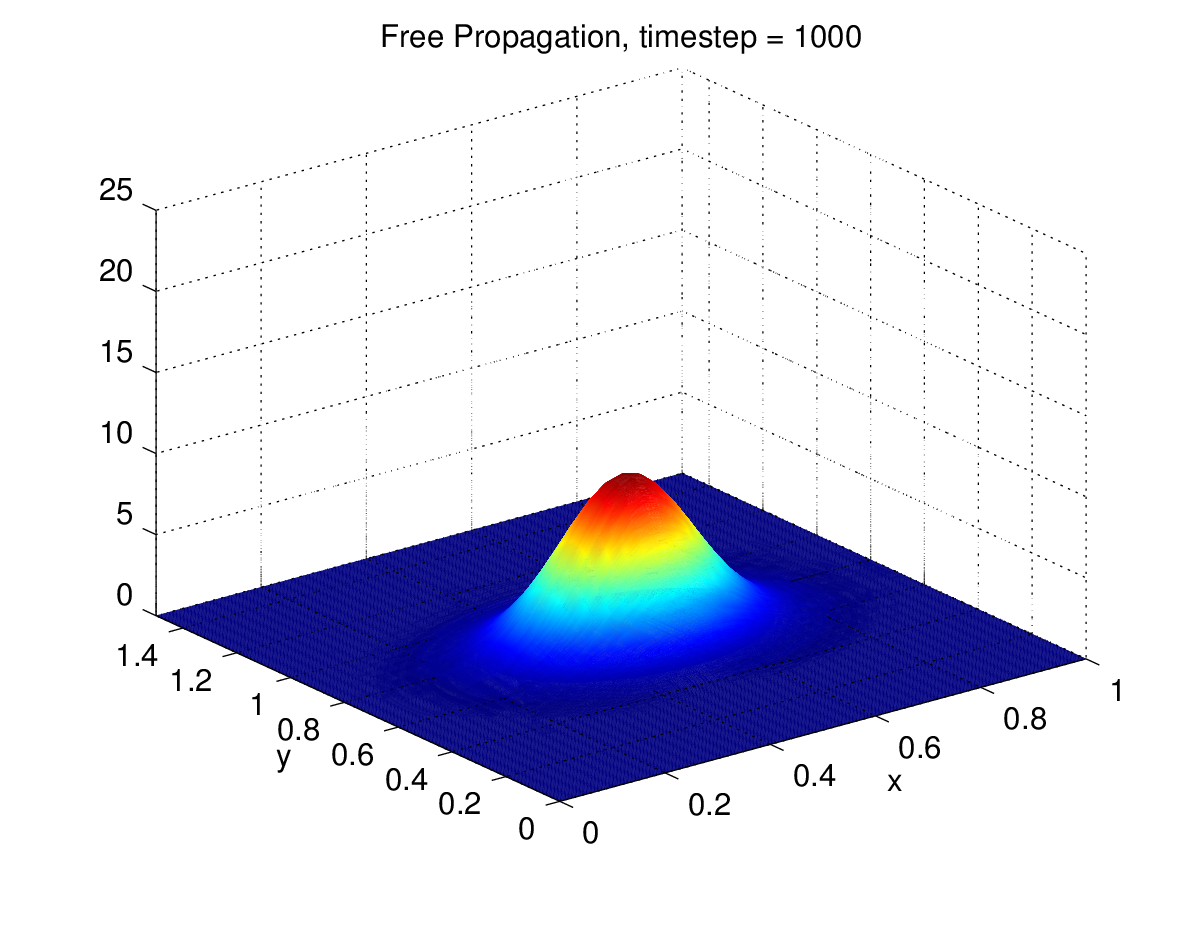
\includegraphics[scale=0.55,trim = 2mm 12mm 12mm 2mm,clip=true]{prop2.png}
\caption{Free propagation, time step = 1000}
\label{fig:p2}
\end{figure}

\begin{figure}[!htbp]
\centering
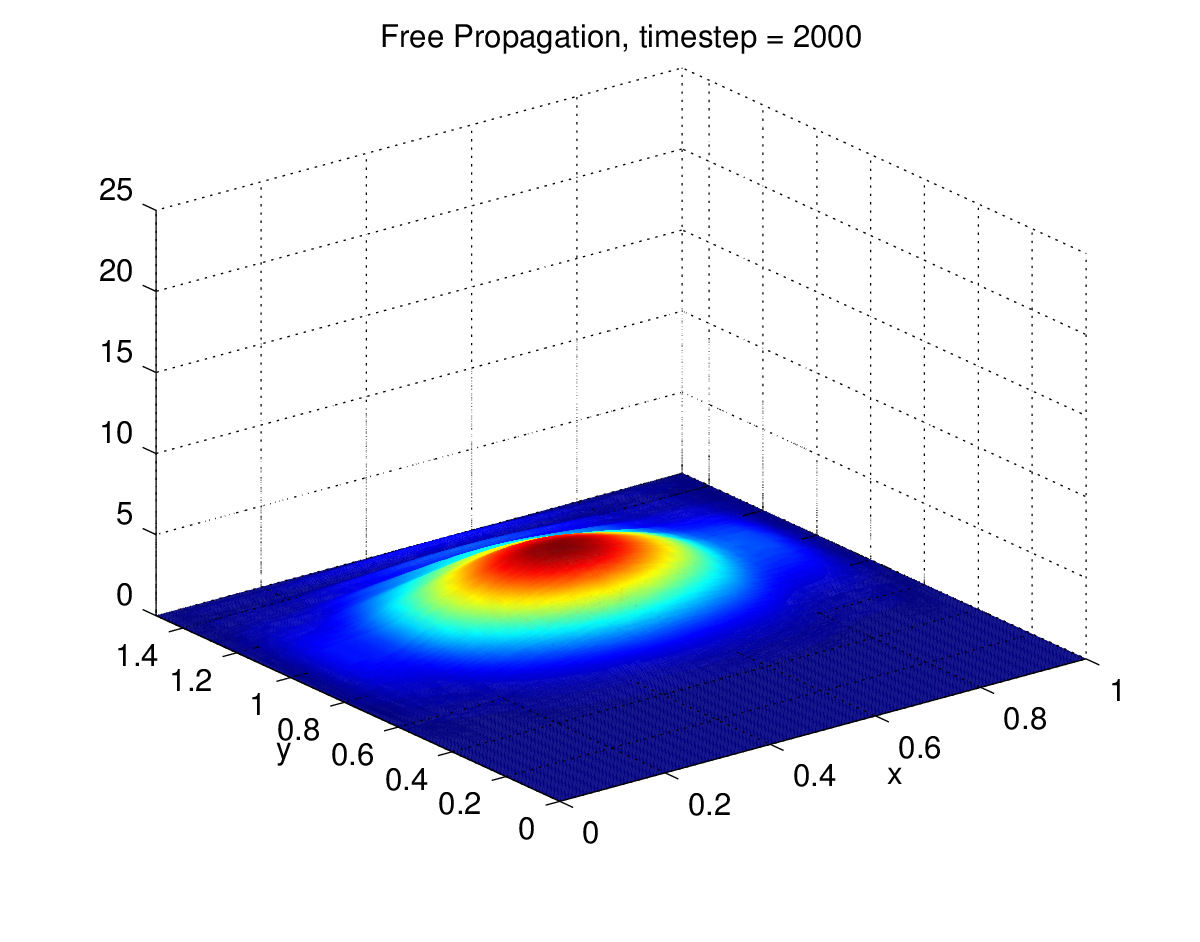
\includegraphics[scale=0.55,trim = 2mm 12mm 12mm 2mm,clip=true]{prop3.png}
\caption{Free propagation, time step = 2000}
\label{fig:p3}
\end{figure}

\begin{figure}[!htbp]
\centering
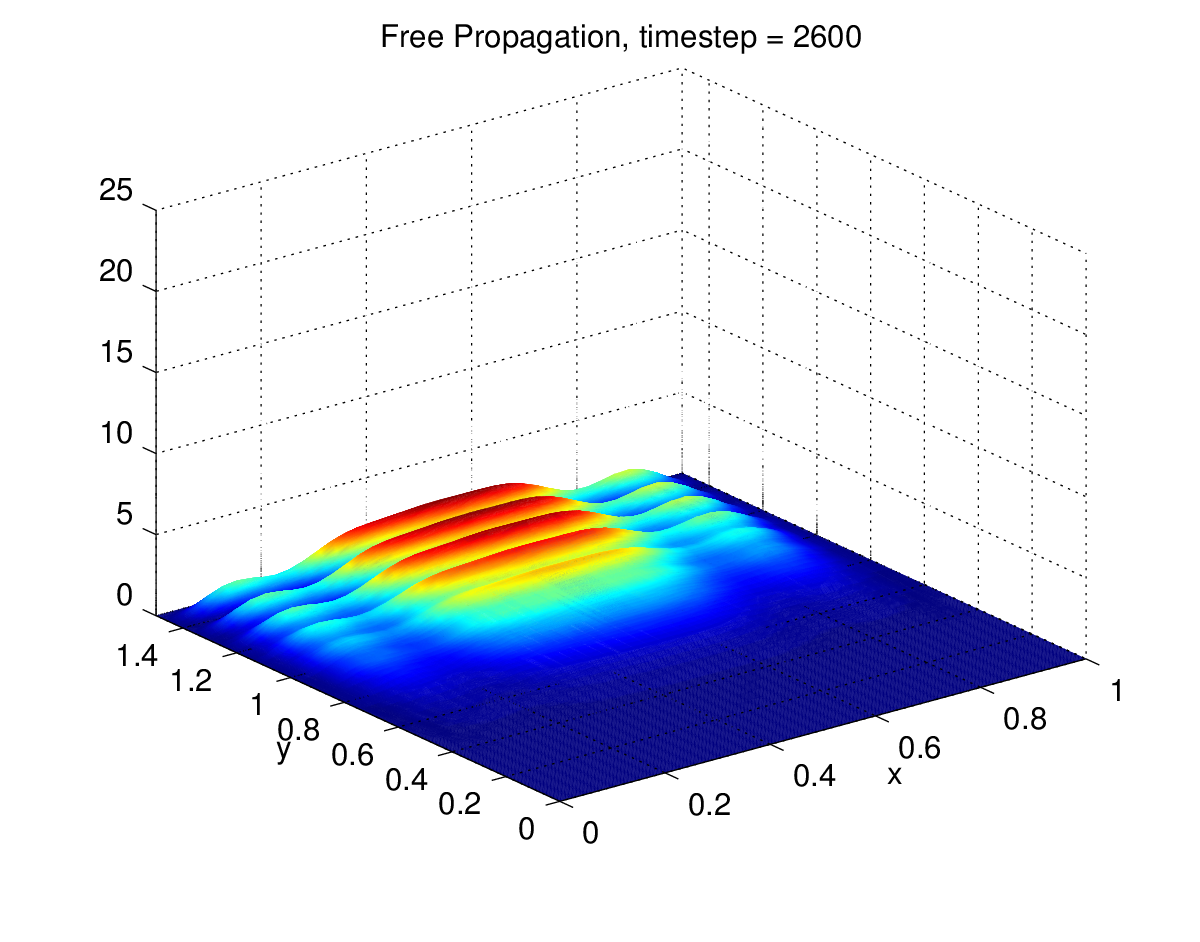
\includegraphics[scale=0.55,trim = 2mm 12mm 12mm 2mm,clip=true]{prop4.png}
\caption{Free propagation, time step = 2600. We see that the wave packet is impinging on the potential wall.}
\label{fig:p3}
\end{figure}

\newpage

\subsection{Gaussian Wave Packet Tunneling}

Next, we attempt to observe tunneling through a large potential barrier.  This simulation can be reproduced by running $examples::run\_cn3()$ from the source code. Here are the parameters for this simulation.:

\begin{center}
    \begin{tabular}{ | l | l  |}
    \hline
    Parameter & Value  \\ \hline
	$k_x$ & 20  \\ \hline
	$k_y$ & 0  \\ \hline    
	$\delta t$ & 5e-6  \\ \hline    
    $\delta x$ & .01  \\ \hline    
    $\delta y$ & .01  \\ \hline 
 	$a$ & 1e3  \\ \hline    
    $\sigma$ & .01  \\ \hline  
    Barrier $x_0$ & 0.75 \\ \hline            
    Solver & Conjugate Gradient  \\ \hline            
    \hline
    \end{tabular}
\end{center}

Note that the potential barrier is defined as a Gaussian, as in the following equation:

\begin{equation}
\begin{split}
V(x) = a\exp( \frac{-(x-x_0)^2}{(2\sigma^2)} )
\end{split}
\end{equation}

This means the potential barrier has a maximum height of 1000, and is tightly focused, in a spatial sense.

The results of this experiment are shown in Figures \ref{fig:b1} - \ref{fig:b3}.  In Figure \ref{fig:b2}, we see the wave packet begin to impinge upon the potential barrier.  In Figure \ref{fig:b3}, it is noticed that some of the waveform has tunneled through the barrier, and some is reflected back.  This result matches the reference work quite well, but note the difference in aspect ratio and colormap.

Also, notice that we have used twice the time step as compared to the reference work, without any ill effects.  This is due the stability of the Crank-Nicholson method.  I was able to complete the simulation using even larger time steps, but convergence was much slower. 


\begin{figure}[!htbp]
\centering
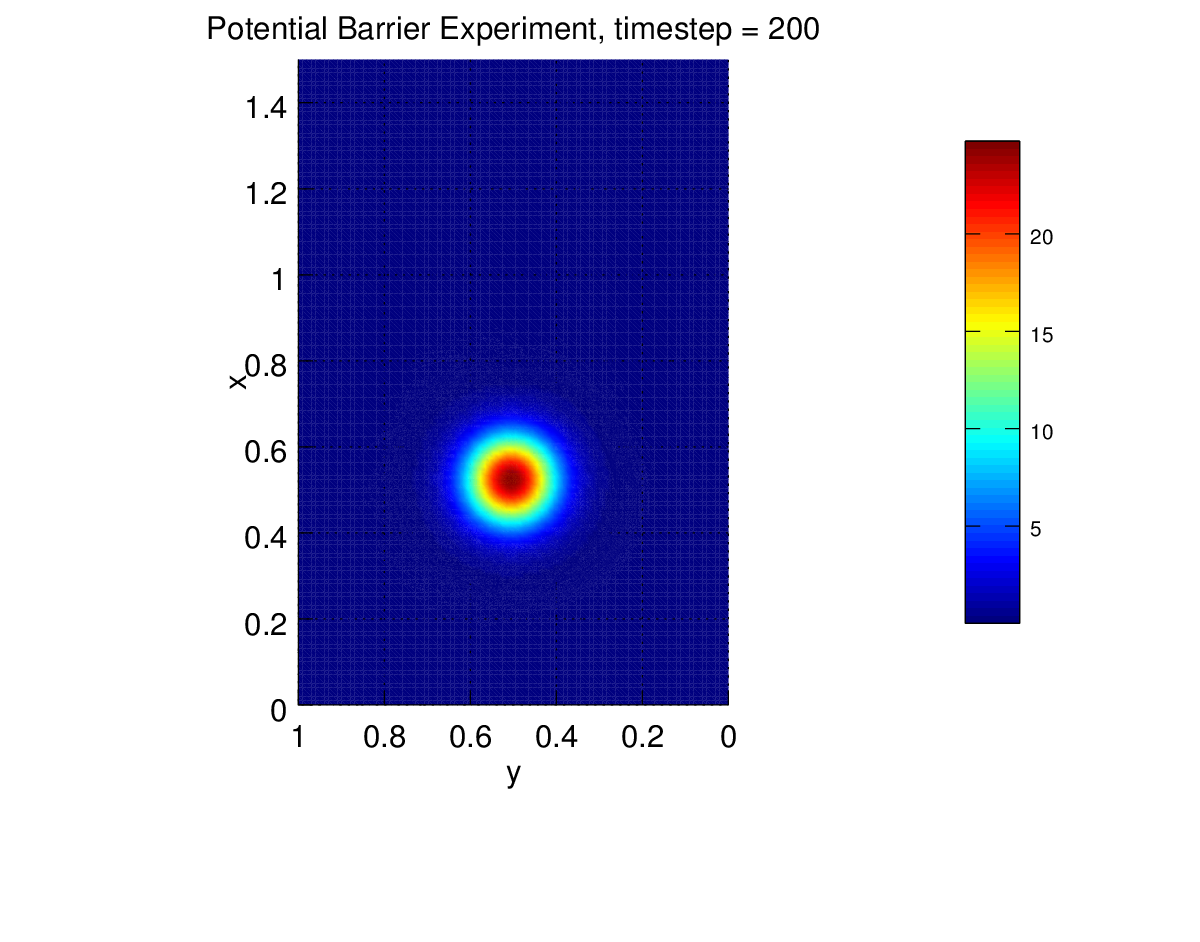
\includegraphics[scale=0.65,trim = 2mm 25mm 2mm 15mm]{barrier1.png}
\caption{Wavepacket moving toward the potential barrier (which is located at $x_0 = 0.75$) }
\label{fig:b1}
\end{figure}

\begin{figure}[!htbp]
\centering
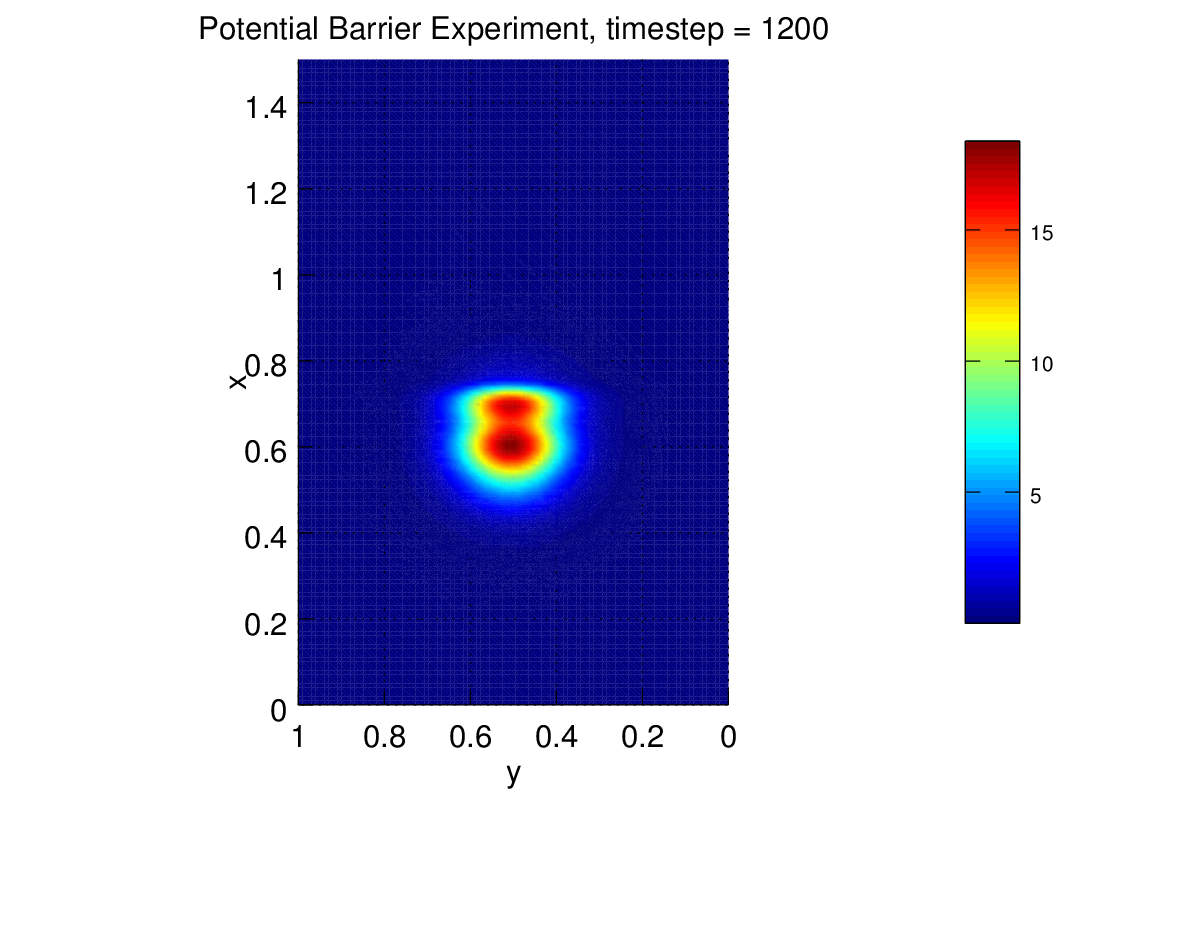
\includegraphics[scale=0.65,trim = 2mm 25mm 2mm 15mm]{barrier2.png}
\caption{Wavepacket impinging upon the barrier.}
\label{fig:b2}
\end{figure}


\begin{figure}[!htbp]
\centering
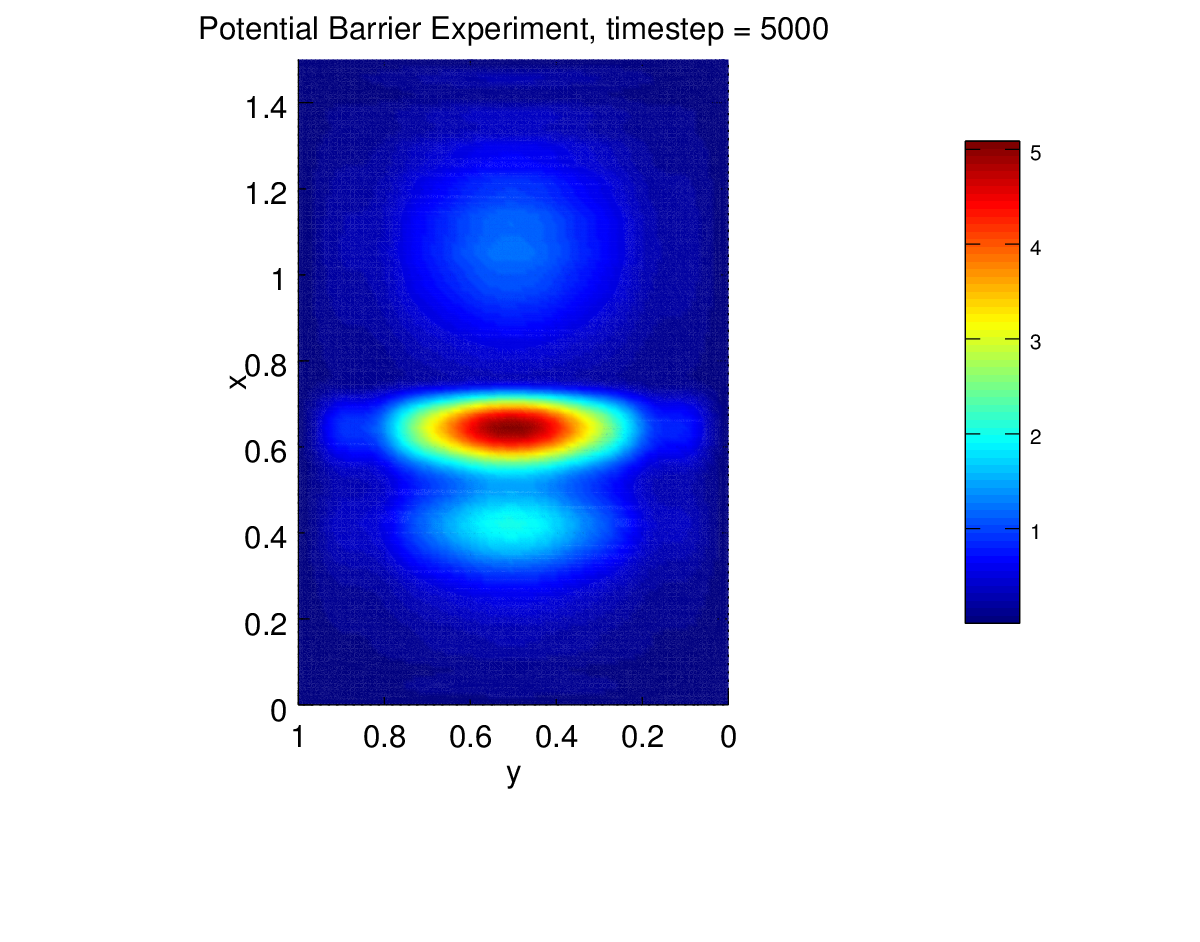
\includegraphics[scale=0.65,trim = 2mm 25mm 2mm 15mm]{barrier3.png}
\caption{In this figure, we see that some of the wavepacket has tunneled through the barrier.}
\label{fig:b3}
\end{figure}

\newpage
\subsection{Double-Slit Experiment}

Finally, we repeat the double-slit experiment from the reference work, which produces an interesting result.  This simulation can be reproduced by running $examples::run\_cn4()$ from the source code. Here are the parameters for this simulation:

\begin{center}
    \begin{tabular}{ | l | l  |}
    \hline
    Parameter & Value  \\ \hline
	$k_x$ & 60  \\ \hline
	$k_y$ & 0  \\ \hline    
	$\delta t$ & 10e-6  \\ \hline    
    $\delta x$ & .01  \\ \hline    
    $\delta y$ & .01  \\ \hline 
 	$a$ & 1e3  \\ \hline    
    $\sigma$ & .01  \\ \hline  
    Barrier $x_0$ & 0.75 \\ \hline            
	Aperture Size & $(2\pi)/60$ \\ \hline            
    Solver & Conjugate Gradient  \\ \hline            
    \hline
    \end{tabular}
\end{center}

Notice that we have again chosen our time step to be twice as large as that of the reference work.  

In Figure \ref{fig:ds3}, we see the domain's potential.  The slits can be observed, as well as the slightly increased potential near the walls of the domain, which serve as our boundary conditions.

Figures \ref{fig:ds1} and \ref{fig:ds2} show the expected diffraction, and match closely with the results produced in \citep{reference}.

\begin{figure}[!htbp]
\centering
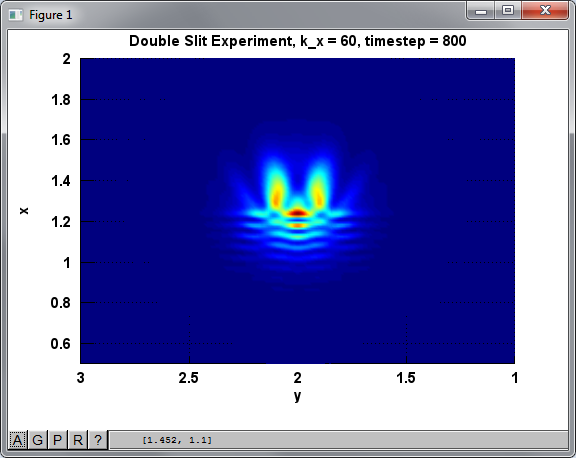
\includegraphics[scale=0.85,trim = 20mm 20mm 20mm 9mm,clip=true]{doubleslit800.png}
\caption{Double slit experiment.  Note that this figure is upside down with respect to the corresponding image in \citep{reference}.}
\label{fig:ds1}
\end{figure}

\begin{figure}[!htbp]
\centering
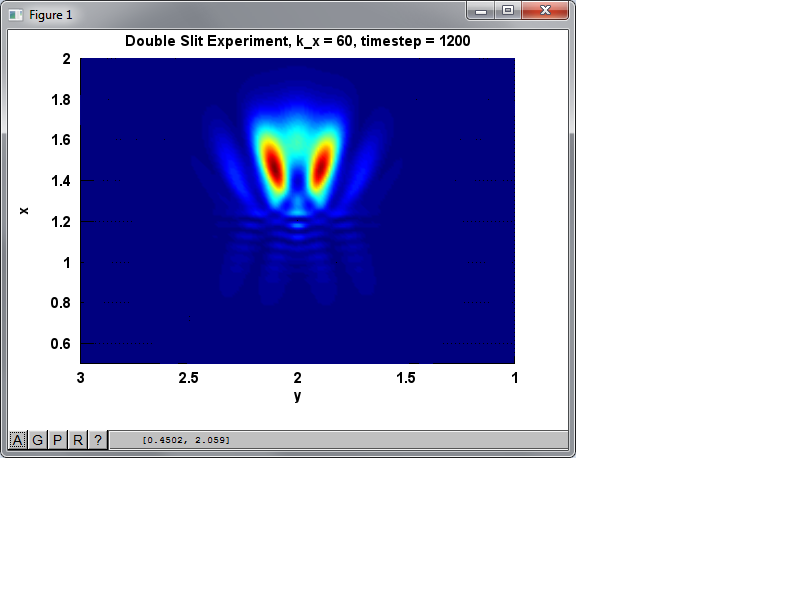
\includegraphics[scale=0.85,trim = 20mm 50mm 70mm 9mm,clip=true]{doubleslit1200.png}
\caption{Double slit experiment}
\label{fig:ds2}
\end{figure}

\begin{figure}[!htbp]
\centering
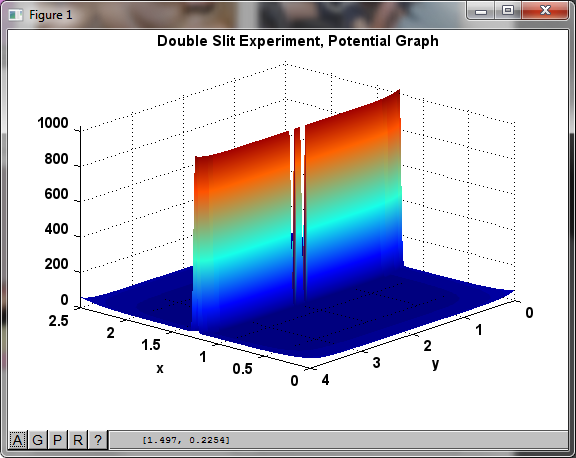
\includegraphics[scale=0.85,trim = 10mm 10mm 4mm 8mm,clip=true]{potential.png}
\caption{Potential for double slit experiment}
\label{fig:ds3}
\end{figure}

Note that while \citep{reference} mentioned that this result took about 30 minutes to produce, the present code was able to complete the simulation within a few minutes.

\section{Future Work}

There are a few items that I'd like to have completed, but could not.

\subsection{Reflection/Transmission Coefficient}

Computing the reflection and transmission coefficients is of practical importance.  In terms of the present code, obtaining the R/T coefficients might look a bit like this:

\begin{itemize}
  \item Instead of keeping track of $\psi$, keep track of $\psi$, and also another $\psi$, which is updated as if no barrier or other potential were present.  
  \item At each time step, compare these two quantities at a specified plane for reflection, and a specified plane for transmission.
  \item At the end of the simulation, compute frequency spectra for reflection and transmission using a Discrete Fourier Transform.
 \end{itemize}

Of course, it is probably more involved than this.

\subsection{Periodic Boundary Conditions}

This should not be too hard, and may be required for R/T coefficients to be precisely correct. Also, I am not completely convinced that the potential well idea used as the boundary condition is totally sufficient. For example, should not tunneling occur through the barrier walls?

\subsection{Higher-Order Explicit Method}

As noted earlier, I did not have much success with the Runge-Kutta method.  It would be important to learn to implement this, or another more stable explicit method.  Since explicit schemes have lower computational complexity than a matrix solution, the Crank-Nicholson scheme used in this work may be unreasonable for very large problems.  
\section{Conclusion}

In this work, we have successfully created a finite difference code to simulate Schrodinger dynamics.  Using this code, we were able to simulate some basic behavior, and match results from the literature.  

We got a lot of mileage out of our rudimentary conjugate gradient solver, and in fact, convergence of the matrix solution was often the limiting factor in choosing a time step.  In other words, other solution methods may converge with even larger time steps, and/or converge more quickly.

\bibliographystyle{plain}
\bibliography{mdbib}

\end{document}



  
